
\documentclass{beamer}
\usetheme{Montpellier} 
\usecolortheme{dolphin} 
\usepackage{tikz}
\usepackage{tkz-berge}
\usepackage{parskip}
\setlength{\parskip}{\smallskipamount} 
\usepackage{amsmath}
\usepackage{array}
\usepackage{fancybox}
\usepackage{mathrsfs}

\title{Extremal Cayley Graphs}
\author{Jordan Blocher, Christopher Linden,  Samantha Hampton}
\date{\today}
\institute[2008]{REU - Texas State}

 \def\ddd{\displaystyle}
 \def\R{\mbox{$\mathbb R$}}
 \def\Q{\mbox{$\mathbb Q$}}
 \def\Z{\mbox{$\mathbb Z$}}
 \def\N{\mbox{$\mathbb N$}}
 \def\C{\mbox{$\mathbb C$}}


\def\Sym{\operatorname{Sym}}
\def\lcm{\operatorname{lcm}}
\def\adj{\operatorname{adj}}
\def\inc{\operatorname{inc}}
\def\Cay{\operatorname{Cay}}
\def\Geom{\operatorname{\cal G}}
\def\diam{\operatorname{diam}}
\def\rank{\operatorname{rank}}


\begin{document}

\frame{\titlepage}
\frame{
	\frametitle{\underline{Introduction to Cayley Graphs}}
\begin{center}
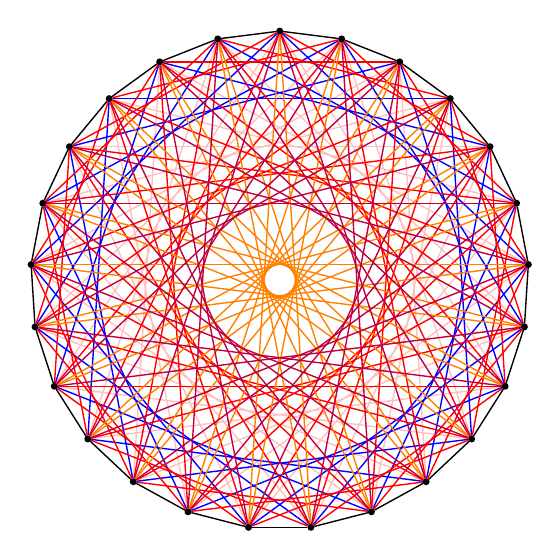
\begin{tikzpicture}[scale=.6]


\GraphInit[vstyle=Simple]
\tikzset{VertexStyle/.append style = {minimum size =2pt, inner sep = 0pt}}


\Vertex[x=187.5pt,y=337.5pt]{0};
\Vertex[x=224.80348307472823pt,y=332.7874741692947pt]{1};
\Vertex[x=259.7630511152573pt,y=318.94600200657953pt]{2};
\Vertex[x=290.1820658893033pt,y=296.8452941132117pt]{3};
\Vertex[x=314.14918882530225pt,y=267.87401924684946pt]{4};
\Vertex[x=330.15847744427305pt,y=233.85254915624213pt]{5};
\Vertex[x=337.2040092642407pt,y=196.91857792939703pt]{6};
\Vertex[x=334.8430876093033pt,y=159.3928028121413pt]{7};
\Vertex[x=323.22405786990294pt,y=123.63310626523908pt]{8};
\Vertex[x=303.0769864163684pt,y=91.88640153769651pt]{9};
\Vertex[x=275.667787843871pt,y=66.14745084375791pt]{10};
\Vertex[x=242.71868290270174pt,y=48.0335271167623pt]{11};
\Vertex[x=206.2999850346457pt,y=38.682794802828326pt]{12};
\Vertex[x=168.70001496535434pt,y=38.682794802828326pt]{13};
\Vertex[x=132.2813170972983pt,y=48.03352711676226pt]{14};
\Vertex[x=99.3322121561291pt,y=66.14745084375782pt]{15};
\Vertex[x=71.92301358363159pt,y=91.88640153769656pt]{16};
\Vertex[x=51.77594213009703pt,y=123.63310626523916pt]{17};
\Vertex[x=40.1569123906967pt,y=159.3928028121413pt]{18};
\Vertex[x=37.795990735759275pt,y=196.91857792939695pt]{19};
\Vertex[x=44.841522555726954pt,y=233.8525491562421pt]{20};
\Vertex[x=60.85081117469775pt,y=267.8740192468495pt]{21};
\Vertex[x=84.81793411069665pt,y=296.8452941132117pt]{22};
\Vertex[x=115.23694888474257pt,y=318.9460020065795pt]{23};
\Vertex[x=150.1965169252717pt,y=332.7874741692946pt]{24};

\SetUpEdge[lw         = .5pt,
            color      = black,
            labelcolor = black]

\Edge(24)(0)
\Edge(0)(1)
\Edge(1)(2)
\Edge(2)(3)
\Edge(3)(4)
\Edge(4)(5)
\Edge(5)(6)
\Edge(6)(7)
\Edge(7)(8)
\Edge(8)(9)
\Edge(9)(10)
\Edge(10)(11)
\Edge(11)(12)
\Edge(12)(13)
\Edge(13)(14)
\Edge(14)(15)
\Edge(15)(16)
\Edge(16)(17)
\Edge(17)(18)
\Edge(18)(19)
\Edge(19)(20)
\Edge(20)(21)
\Edge(21)(22)
\Edge(22)(23)
\Edge(23)(24)

\SetUpEdge[lw         = .5pt,
            color      =pink,
            labelcolor = black]

\Edge(0)(8)
\Edge(2)(10)
\Edge(4)(12)
\Edge(6)(14)
\Edge(8)(16)
\Edge(10)(18)
\Edge(12)(20)
\Edge(14)(22)
\Edge(16)(24)
\Edge(18)(1)
\Edge(20)(3)
\Edge(22)(5)
\Edge(24)(7)
\Edge(1)(9)
\Edge(3)(11)
\Edge(5)(13)
\Edge(7)(15)
\Edge(9)(17)
\Edge(11)(19)
\Edge(13)(21)
\Edge(15)(23)
\Edge(17)(0)
\Edge(19)(2)
\Edge(21)(4)
\Edge(23)(6)

\SetUpEdge[lw         = .5pt,
            color      =blue,
            labelcolor = black]

\Edge(0)(6)
\Edge(6)(12)
\Edge(12)(18)
\Edge(18)(24)
\Edge(24)(5)
\Edge(5)(11)
\Edge(11)(17)
\Edge(17)(23)
\Edge(23)(4)
\Edge(4)(10)
\Edge(10)(16)
\Edge(16)(22)
\Edge(22)(3)
\Edge(3)(9)
\Edge(9)(15)
\Edge(15)(21)
\Edge(21)(2)
\Edge(2)(8)
\Edge(8)(14)
\Edge(14)(20)
\Edge(20)(1)
\Edge(1)(7)
\Edge(7)(13)
\Edge(13)(19)
\Edge(19)(0)

\SetUpEdge[lw         = .5pt,
            color      =red,
            labelcolor = black]

\Edge(0)(4)
\Edge(4)(8)
\Edge(8)(12)
\Edge(12)(16)
\Edge(16)(20)
\Edge(20)(24)
\Edge(24)(3)
\Edge(3)(7)
\Edge(7)(11)
\Edge(11)(15)
\Edge(15)(19)
\Edge(19)(23)
\Edge(23)(2)
\Edge(2)(6)
\Edge(6)(10)
\Edge(10)(14)
\Edge(14)(18)
\Edge(18)(22)
\Edge(22)(1)
\Edge(1)(5)
\Edge(5)(9)
\Edge(9)(13)
\Edge(13)(17)
\Edge(17)(21)
\Edge(21)(0)
\Edge(0)(9)
\Edge(9)(18)
\Edge(18)(2)
\Edge(2)(11)
\Edge(11)(20)
\Edge(20)(4)
\Edge(4)(13)
\Edge(13)(22)
\Edge(22)(6)
\Edge(6)(15)
\Edge(15)(24)
\Edge(24)(8)
\Edge(8)(17)
\Edge(17)(1)
\Edge(1)(10)
\Edge(10)(19)
\Edge(19)(3)
\Edge(3)(12)
\Edge(12)(21)
\Edge(21)(5)
\Edge(5)(14)
\Edge(14)(23)
\Edge(23)(7)
\Edge(7)(16)
\Edge(16)(0)


\SetUpEdge[lw         = .5pt,
            color      = orange,
            labelcolor = black]

\Edge(24)(12)
\Edge(0)(13)
\Edge(1)(14)
\Edge(2)(15)
\Edge(3)(16)
\Edge(4)(17)
\Edge(5)(18)
\Edge(6)(19)
\Edge(7)(20)
\Edge(8)(21)
\Edge(9)(22)
\Edge(10)(23)
\Edge(11)(24)
\Edge(12)(0)
\Edge(13)(1)
\Edge(14)(2)
\Edge(15)(3)
\Edge(16)(4)
\Edge(17)(5)
\Edge(18)(6)
\Edge(19)(7)
\Edge(20)(8)
\Edge(21)(9)
\Edge(22)(10)
\Edge(23)(11)


\SetUpEdge[lw         = .5pt,
            color      = purple,
            labelcolor = black]

\Edge(24)(9)
\Edge(0)(10)
\Edge(1)(11)
\Edge(2)(12)
\Edge(3)(13)
\Edge(4)(14)
\Edge(5)(15)
\Edge(6)(16)
\Edge(7)(17)
\Edge(8)(18)
\Edge(9)(19)
\Edge(10)(20)
\Edge(11)(21)
\Edge(12)(22)
\Edge(13)(23)
\Edge(14)(24)
\Edge(15)(0)
\Edge(16)(1)
\Edge(17)(2)
\Edge(18)(3)
\Edge(19)(4)
\Edge(20)(5)
\Edge(21)(6)
\Edge(22)(7)
\Edge(23)(8)

\end{tikzpicture}
\end{center}

\begin{itemize}
		\item<1->
\begin{center}
Cay($\mathbb{Z}_{25}$, \{$\pm$1,$\pm$4,$\pm$6,$\pm$8, $\pm10$, $\pm$13\})     
\end{center}
                 
\end{itemize}
}

\frame {
	\frametitle{\underline{Introduction to Cayley Graphs}}
	\only<1>{
	\begin{itemize}
                  \item<1-> Definition:  Let $\Gamma$ be a finite group with a subset $\mathscr{A}$. The {\emph{Cayley digraph}}, denoted $\Cay(\Gamma,\mathscr{A})$, is a digraph with vertex set $\Gamma$, such that (x,y) is a directed edge if and only if $yx^{-1} \in \mathscr{A}$.

		\item<1->\emph{Cayley digraphs} are vertex transitive.
		\item<1->The Cayley digraph of a finit cyclic group is called a circulant graph.  Our project focuses on circulant graphs.

	\end{itemize}
}
}

\frame {
	\frametitle{\underline{Introduction to Cayley Graphs}}
	\only<1>{
	\begin{itemize}
                  \item<1-> For a positive integer $d$ and a subset of integers $\mathscr{A}$ we define :
\begin{align*}
m(d,\mathscr{A}) &=\max\{m | \diam(\Cay(\mathbb{Z}_m,\mathscr{A})) \leq d\} \text{,} \\
\end{align*}
\item<1-> For positive integers $d$ and $k$ we define
\begin{align*}
m(d,k) &= \max_{|A| = k}\{m(d,A)  \}.
\end{align*}
	\end{itemize}
}
}


\frame{
	\frametitle{\underline{Introduction to Cayley Graphs}}
	\only<1>{
	\begin{itemize}
                  \item<1-> Current known values include:
\begin{align*}
m(1,k) &= k+1,
\\
\textcolor{blue}{m(2,k)} &\geq \textcolor{blue}{\frac{37}{121}k^2 + O(k)},
\\
m(d,1) &= d+1\text{, and}
\\
m(d,2) &= \left\lfloor \frac{d(d+4)}{3} \right\rfloor+1 \text{ for all } d\geq2.
\end{align*}

	\end{itemize}
}
}

\frame{
	\frametitle{\underline{Finding lower bounds on m(d,k)}}
	\only<1>{
	\begin{itemize}
                  \item<1-> For a (small) fixed k, we can give a set $\mathscr{A}$ the $k$ elements of which are written in terms of $d$.  If we can prove that $d\mathscr{A}$ always contains $\Z_m$ for some $m$, also a function of $d$, then we have a lower bound for $m(d,k)$.
                  \item<1-> For example, the set $\mathscr{A} = \{1, 3d -8\lfloor{\frac{d}{4}}\rfloor +5, \lfloor{\frac{d}{4}}\rfloor(3d -8\lfloor{\frac{d}{4}}\rfloor +5) +d - 3\lfloor{\frac{d}{4}}\rfloor \}$ generates $m = \frac{d^3}{16} + \frac{3d^2}{8} + O(d)$, so $m(d,3) \ge \frac{d^3}{16} + O(d^2)$.

	\end{itemize}
}
}

\frame{
	\frametitle{\underline{Finding lower bounds on m(d,k)}}
	\only<1>{
	\begin{itemize}
                  \item<1-> If the sets $\mathscr{A}$ and values $m$ are of a particular form, it is possible to have a computer check whether or not  $d\mathscr{A} \supset \Z_m$. 
                  \item<1-> We can then (in theory) have the computer loop though all possible generating sets and moduli of this particular form to search for new lower bounds.
                  \item<1->In practice, this may be computationally infeasible.

	\end{itemize}
}
}
\frame{
	\frametitle{\underline{The Algorithm}}
	\only<1>{
	\begin{itemize}
                  \item<1-> ??
                  
	\end{itemize}
}
}

\frame{
	\frametitle{\underline{The General Case}}
	\only<1>{
	\begin{itemize}
                  \item<1-> One of the reasons we are interested in lower bounds on $m(d,k)$ for specific values of $k$ is because we can use them to obtain a lower bound for arbitrary $k$ as $d \to \infty$.
                  \item<1-> We use the inequality
\[
	m(d_1+d_2,k_1+k_2) \ge m(d_1,k_1)m(d_2,k_2)
\]
to establish these general case bounds.
				\item<1-> We can also use it to find bounds for arbitrary $d$ as $k \to \infty$.                
	\end{itemize}
}
}

\frame{
	\frametitle{\underline{The General Case: example proof}}
	\only<1>{
	\begin{itemize}
                  \item<1-> Using our $m(2,k)$ result, we prove a lower bound on $m(d,k)$ as $k \to \infty$. 
                  \item<1-> Claim: For any integer $d \geq 2$, as $k \to \infty$, we have 
\[
m(d,k) \geq \left(\frac{148}{121}\right)^{\lfloor \frac{d}{2}\rfloor}\left(\frac{k}{d}\right)^d + O(k^{d-1}).
\]
                                
	\end{itemize}
}
}

\frame{
	\frametitle{\underline{The General Case: example proof}}
	\only<1>{
	\begin{itemize}
                  \item<1-> Let $d = 2q +r$ where $q =\displaystyle\left \lfloor \frac{d}{2}\right\rfloor$ and $k = du +v$ where $u =\displaystyle \left \lfloor \frac{k}{d}\right\rfloor$. We separate the calculation into two cases.
                                
	\end{itemize}
}
}

\frame{
	\frametitle{\underline{The General Case: example proof}}
	\only<1>{
	\begin{itemize}
                  \item<1-> Case 1: If $r = 0$, then
\begin{align*}
m(d,k) &= m(2q, du +v)\\
&= m(2q, (2q)u +v)\\
&\geq m(2q, 2qu) \geq m(2, 2u)^q\\
&\geq \left(\frac{37}{121}(2u)^2+ O(u)\right)^q \\
&= \left(\frac{148}{121} \left(\frac{k-v}{d}\right) ^2+ O(u)\right)^{ \frac{d}{2}}\\
&= \left(\frac{148}{121}\right)^{ \frac{d}{2}}\left(\frac{k}{d}\right)^d + O(k^{d-1})
\end{align*}
                                
	\end{itemize}
}
}

\frame{
	\frametitle{\underline{The General Case: example proof}}
	\only<1>{
	\begin{itemize}
                  \item<1-> Case 2: If $r = 1$, then
\begin{align*}
m(d,k) &= m(2q+1, du +v) = m(2q+1, (2q+1)u +v)\\
&\geq m(2q+1, 2qu + u) \geq m(2, 2u)^q \cdot m(1,u)\\
&\geq \left(\frac{37}{121}(2u)^2+ O(u)\right)^q \cdot (u+1) \\
&= \left(\frac{148}{121} u^2 + O(u)\right)^{ \frac{d-1}{2}} \cdot (u+1)\\
&= \left(\frac{148}{121}^{ \frac{d-1}{2}} u ^{d-1}+ O(u^{d-2})\right) \cdot (u+1)\\
&= \frac{148}{121}^{ \frac{d-1}{2}} u ^{d}+ O(u^{d-1})\\
&= \left(\frac{148}{121}\right)^{ \frac{d-1}{2}}\left(\frac{k}{d}\right)^d + O(k^{d-1})
\end{align*}                            
	\end{itemize}
}
}

\frame{
	\frametitle{\underline{The General Case: example proof}}
	\only<1>{
	\begin{itemize}
                  \item<1-> Hence 
\[
m(d,k) \geq \left(\frac{148}{121}\right)^{\lfloor \frac{d}{2}\rfloor}\left(\frac{k}{d}\right)^d + O(k^{d-1}).
\]
                           
	\end{itemize}
}
}

\frame{
	\frametitle{\underline{Open Problems}}
	\only<1>{
	\begin{itemize}
                  \item<1->  For $n(d,k)$ it is known that for every positive integer $k$ the limit 
\[
\lim_{d \to \infty}{\frac{n(d,k)}{d^k}}
\]
exists, and the value is known for $k = 1,$ $2$ and $3$.  It is not known whether or not 
\[
\lim_{d \to \infty}{\frac{m(d,k)}{d^k}}
\]
exists for every k, and the value is only known for $k = 1$ and $2$. \\

                           
	\end{itemize}
}
}

\frame{
	\frametitle{\underline{Open Problems}}
	\only<1>{
	\begin{itemize}
                  \item<1-> The existence or values of the limits
\[
\lim_{d \to \infty}{\frac{m(d,k)}{n(d,k)}} \text{ and}
\lim_{k \to \infty}{\frac{m(d,k)}{n(d,k)}}
\]
are also of interest.
                           
	\end{itemize}
}
}

\frame{
	\frametitle{\underline{Open Problems}}
	\only<1>{
	\begin{itemize}
                  \item<1-> We may define the undirected version of our extremal function $M(d,k)$ to be the largest $M$ such that there exists of symmetric set $\mathscr{A}$ of $k$ elements and their additive inverses such that $\diam(Cay(\Z_M,\mathscr{A})) \leq d$.  Little is known about $M(d,k)$, for fixed $d$ and $k \geq 3$. 
                  \item<1-> We may also define the average version of our extremal function $\bar{m}(d,k)$ to be the largest $m$ such that there exists a set $\mathscr{A}$ of $k$ elements such that the average distance between any two vertices in $Cay(\Z_m,\mathscr{A})$ is less than $d$. New lower bounds for $k \geq 3$ would be interesting for this function as well.

                           
	\end{itemize}
}
}



\end{document}
